\section{Fanny Shafira Damayanti (1174069)}
\subsection{Buku}
Belum Lunas
\subsection{Pengertian Sistem Informasi Geografis}
Sistem Informasi Geografis merupakan system yang memiliki kemampuan untuk menyimpan, membangun, mengelola semua informasi yang bereferensi geografis.
\subsection{Sejarah}
Awal dikenalnya SIG tidak lepas dari adanya kemajuan dalam bidang teknologi terutama komputer. Selama perang dunia kedua pemrosesan data mengalami kemajuan yang pesat terutama untuk memenuhi kebutuhan militer dalam memprediksi trayektori balistik. Pada awal tahun 1960-an perkembangan dalam ilmu komputer semakin pesat dan siap digunakan untuk bidang lain di luar militer. Para ahli meteorologi, geologi, dan geofisika mulai menggunakan komputer dalam pembuatan peta.
Tahun 1963 di Kanada muncul CGIS (Canadian Geographic Information System), dan selanjutnya menjadi SIG pertama di dunia. Dua tahun kemudian di Amerika Serikat beroperasi sistem serupa bernama MIDAS yang digunakan untuk memproses data-data sumber daya alam.
Seiring dengan berkembangnya teknologi, GIS juga mengalami perubahan ke arah yang lebih baik. Berikut adalah sejarah perkembangan GIS dari masa ke masa :
\begin{itemize}
\item 35000 tahun yang lalu, di dinding gua Lascaux, Perancis, para pemburu Cro-Magnon menggambar hewan mangsa mereka, juga garis yang dipercaya sebagai rute migrasi hewan-hewan tersebut. Catatan awal ini sejalan dengan dua elemen struktur pada sistem informasi gegrafis modern sekarang ini, arsip grafis yang terhubung ke database atribut.

\item Pada tahun 1700-an teknik survey modern untuk pemetaan topografis diterapkan, termasuk juga versi awal pemetaan tematis, misalnya untuk keilmuan atau data sensus.

\item Awal abad ke-20 memperlihatkan pengembangan “litografi foto” dimana peta dipisahkan menjadi beberapa lapisan (layer). Perkembangan perangkat keras komputer yang dipacu oleh penelitian senjata nuklir membawa aplikasi pemetaan menjadi multifungsi pada awal tahun 1960-an.

\item Tahun 1967 merupakan awal pengembangan SIG yang bisa diterapkan di Ottawa, Ontario oleh Departemen Energi, Pertambangan dan Sumber Daya. Dikembangkan oleh Roger Tomlinson, yang kemudian disebut CGIS (Canadian GIS – SIG Kanada), digunakan untuk menyimpan, menganalisis dan mengolah data yang dikumpulkan untuk Inventarisasi Tanah Kanada (CLI – Canadian land Inventory) – sebuah inisiatif untuk mengetahui kemampuan lahan di wilayah pedesaan Kanada dengan memetakaan berbagai informasi pada tanah, pertanian, pariwisata, alam bebas, unggas dan penggunaan tanah pada skala 1:250000. Faktor pemeringkatan klasifikasi juga diterapkan untuk keperluan analisis.

\item GIS dengan gvSIG.CGIS merupakan sistem pertama di dunia dan hasil dari perbaikan aplikasi pemetaan yang memiliki kemampuan timpang susun (overlay), penghitungan, pendijitalan/pemindaian (digitizing/scanning), mendukung sistem koordinat national yang membentang di atas benua Amerika , memasukkan garis sebagai arc yang memiliki topologi dan menyimpan atribut dan informasi lokasional pada berkas terpisah. Pengembangya, seorang geografer bernama Roger Tomlinson kemudian disebut “Bapak SIG”.

\item CGIS bertahan sampai tahun 1970-an dan memakan waktu lama untuk penyempurnaan setelah pengembangan awal, dan tidak bisa bersaing denga aplikasi pemetaan komersil yang dikeluarkan beberapa vendor seperti Intergraph. Perkembangan perangkat keras mikro komputer memacu vendor lain seperti ESRI dan CARIS berhasil membuat banyak fitur SIG, menggabung pendekatan generasi pertama pada pemisahan informasi spasial dan atributnya, dengan pendekatan generasi kedua pada organisasi data atribut menjadi struktur database. Perkembangan industri pada tahun 1980-an dan 1990-an memacu lagi pertumbuhan SIG pada workstation UNIX dan komputer pribadi. Pada akhir abad ke-20, pertumbuhan yang cepat di berbagai sistem dikonsolidasikan dan distandarisasikan menjadi platform lebih sedikit, dan para pengguna mulai mengekspor menampilkan data SIG lewat internet, yang membutuhkan standar pada format data dan transfer. 

\end{itemize}

\subsection{Koordinat}
\begin{itemize}
\item Garis Lintang (Latitude)
\item Garis Lintang (Latitude)
\begin{figure}[H]
	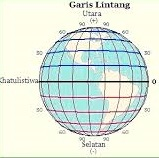
\includegraphics[width=4cm]{figures/Tugas1/1174069/lintang.jpg}
	\centering
	\caption{Gambar Garis Lintang}
\end{figure}
Garis lintang merupakan garis yang menentukan lokasi bumi terhadap garis khatulistiwa (utara atau selatan). 

\item Garis Bujur (Longtitude)
\begin{figure}[H]
	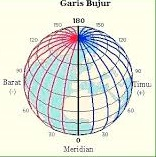
\includegraphics[width=4cm]{figures/Tugas1/1174069/bujur.jpg}
	\centering
	\caption{Gambar Garis Bujur}
\end{figure}
Garis Bujur, menggambarkan lokasi sebuah tempat di timur atau barat Bumi dari sebuah garis utara-selatan yang disebut Meridian Utama. 
\end{itemize}

\subsection{Data Geospasial}
UU No. 4 Tahun 2011 Tentang Informasi Geospasial pasal 1-4 menerangkan, spasial adalah aspek keruangan suatu objek atau  kejadian yang mencakup lokasi, letak, dan posisinya. Geospasial atau ruang kebumian adalah aspek keruangan yang menunjukkan lokasi, letak, dan posisi suatu objek atau kejadian yang berada di bawah, pada, atau di atas permukaan bumi yang dinyatakan dalam sistem koordinat tertentu. Data Geospasial yang selanjutnya disingkat “DG”, adalah data tentang lokasi geografis, dimensi atau ukuran, dan/atau karakteristik objek alam dan/atau buatan manusia yang berada di bawah, pada, atau di atas permukaan bumi. Informasi Geospasial yang selanjutnya disingkat IG adalah DG yang sudah diolah sehingga dapat digunakan sebagai alat bantu dalam perumusan kebijakan, pengambilan keputusan, dan/atau pelaksanaan kegiatan yang berhubungan dengan ruang kebumian.

Contoh data spasial antara lain letak suatu wilayah, posisi sumber minyak bumi,dsb. Bentuk-bentuk data spasial : titik (dot), contoh: posisi terminal; garis (poly line), contoh: jaringan jalan raya; dan area (polygon), contoh: wilayah kecamatan. Contoh data atribut misalnya kepadatan penduduk, jenis tanah, dsb. Bentuk-bentuk data atribut adalahdata kuantitatif (angka-angka/statistik), contoh: jumlah penduduk dan data kualitatif (kualitas/mutu), contoh: tingkat kesuburan tanah.

Jenis-Jenis Data Geospasial
\begin{itemize}
\item Data Vektor
Data vektor adalah data yang direpresentasikan sebagai suatu mosaik berupa garis (arc/line), polygon (daerah yang dibatasi oleh garis yang berawal dan berakhir pada titik yang sama), titik/point (node yang mempunyai label), dan nodes (merupakan titik perpotongan antara dua buah garis). Keuntungan utama dari format data vektor adalah ketepatan dalam merepresentasikan fitur titik, batasan dan garis lurus.

Kegunaan Data Vektor untuk analisa yang membutuhkan ketepatan posisi, misalnya pada basis data batas-batas kadaster. Contoh penggunaan lainnya adalah untuk mendefinisikan hubungan spasial dari beberapa fitur. Kelemahan data vektor yang utama adalah ketidakmampuannya dalam mengakomodasi perubahan gradual.

\item Data Raster
Data raster adalah data yang dihasilkan dari penginderaan jauh. Data Raster sering disebut juga dengan sel grid. Pada data raster, obyek geografis direpresentasikan sebagai struktur sel grid yang disebut dengan pixel (picture element). Pada data raster, resolusi (definisi visual) tergantung pada ukuran pixel-nya. Dengan kata lain, resolusi pixel menggambarkan ukuran sebenarnya di permukaan bumi yang diwakili oleh setiap pixel pada citra.

Semakin kecil ukuran permukaan bumi yang direpresentasikan oleh satu sel, semakin tinggi resolusinya. Data raster sangat baik untuk merepresentasikan batas-batas yang berubah secara gradual, seperti jenis tanah, kelembaban tanah, vegetasi, suhu tanah, dan sebagainya. Kelemahan utama dari data raster adalah besarnya ukuran file; semakin tinggi resolusi grid-nya semakin besar pula ukuran filenya.

Masing-masing format data mempunyai kelebihan dan kekurangan. Pemilihan format data yang digunakan sangat tergantung pada tujuan penggunaan, data yang tersedia, volume data yang dihasilkan, ketelitian yang diinginkan, serta kemudahan dalam analisa. Data vektor relatif lebih ekonomis dalam hal ukuran file dan presisi dalam lokasi, tetapi sangat sulit untuk digunakan dalam komputasi matematik. Sebaliknya, data raster biasanya membutuhkan ruang penyimpanan file yang lebih besar dan presisi lokasinya lebih rendah, tetapi lebih mudah digunakan secara matematis.

\item Titik (dimensi nol - point)
Titik adalah representasi grafis atau geometri yang paling sederhana bagi objek spasial. Representasi ini tidak memiliki dimensi, tetapi dapat diidentifikasikan di atas peta dan dapat ditampilkan pada layar monitor dengan menggunakan simbol-simbol tertentu. Perlu dipahami juga bahwa skala peta akan menentukan apakah suatu objek akan ditampilkan sebagai titik atau polygon. Pada peta skala besar, unsur-unsur bangunan akan ditampilkan sebagai polygon, sedangkan pada skala kecil akan ditampilkan sebagai unsur-unsur titik.
Format titik : koordinat tunggal, tanpa panjang, tanpa luasan.
Contoh : lokasi kecelakaan, letak pohon

\item Garis (satu dimensi – line atau polyline)
Garis adalah bentuk geometri linier yang akan menghubungkan paling sedikit dua titik dan digunakan untuk merepresentasikan objek-objek yang berdimensi satu. Batas-batas objek geometri polygon juga merupakan garis-garis, demikian pula dengan jaringan listrik, jaringan komunikasi, pipa air minum, saluran buangan, dan utility lainnya dapat direpresentasikan sebagai objek dengan bentuk geometri garis. Hal ini akan bergantung pada skala peta yang menjadi sumbernya atau skala representasi akhirnya.

Format : Koordinat titik awal dan akhir, mempunyai panjang tanpa luasan.
Contoh : jalan, sungai, utility

\item Polygon (dua dimensi – area)
Geometri polygon digunakan untuk merepresentasikan objek-objek dua dimensi. Unsurunsur spasial seperti danau, batas propinsi, batas kota, batas persil tanah milik adalah beberapa contoh tipe entitas dunia nyata yang pada umumnya direpresentasikan sebagai objek-objek dengan geometri polygon. Meskipun demikian, representasi ini masih akan bergantung pada skala petanya atau sajian akhirnya.

Format : Koordinat dengan titik awal dan akhir sama, mempunyai panjang dan luasan.
Contoh : Tanah persil, bangunan

\end{itemize}
\subsection{Link}
https://youtu.be/m0sEiWnj3Aw

\subsection{Plagiarism}
\subsection{Plagiarism}
\begin{figure}[H]
	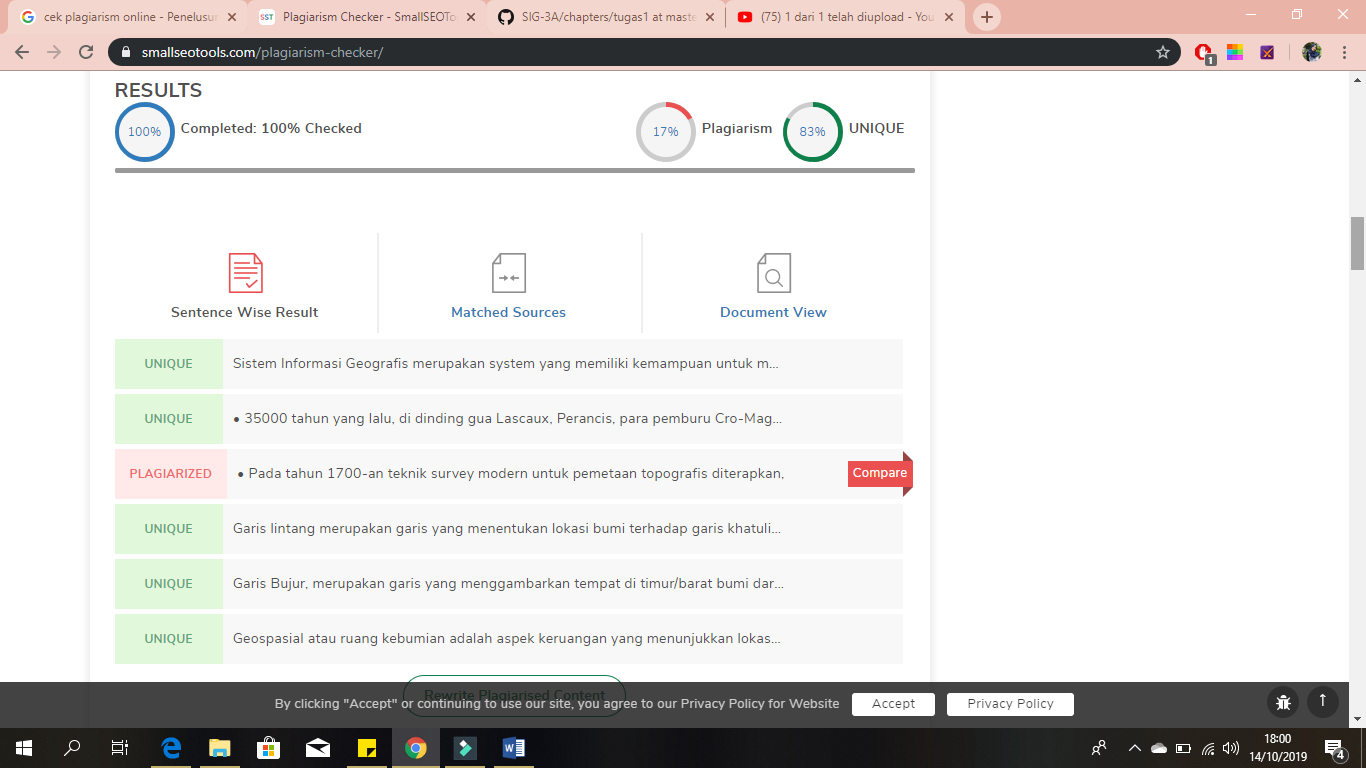
\includegraphics[width=4cm]{figures/Tugas1/1174069/plagiarism.png}
	\centering
	\caption{Gambar Plagiat}
\end{figure}

